\subsection{General information}
The Transient Array Radio Telescope, or TART, is a 24 element aperture synthesis radio telescope. It was originally designed at the University of Otago, New Zealand as a test bench for creating new imaging algorithms. It is also a survey instrument for transient events\cite{DESIGN_TART}. The interferometer operates at a frequency of 1.575 GHz on the L1 band, which is free from interference.
\\
TART consists of a RESTful API, this allows the user to send HTTP requests to the API and receive information back, such as the current visibilities of the Interferometer or the Latitude and frequency that the Interferometer is operating at.\cite{CALIBRATION_TART}\\
Both TART's hardware and software is part of an open source project and the University of Stellenbosch has one installed on the Electrical Engineering building roof, under the supervision of Dr. DJ Ludick.
% Ask Dr. Ludick for a paper
% Explain what TART is

\subsection{How it works}
TART consists of 4 tiles that are 1m$^2$ in size, each with 6 antennas mounted on them, Each antenna is mounted on a 50cm length of PVC pipe. The antennas connect to a radio hub module which is in turn connected to a central telescope control board\cite{LAYOUT_TART}.

The telescope control board, or base station, consists of a power supply, a local oscillator, a FPGA and a miniature ARM based computer. The base station also contains a Raspberry Pi Model 2 which is used for data processing and storage. The base station also supplies power to all of the radio hub modules\cite{CALIBRATION_AND_SYNTHESIS_TART}.

The radio hub module is designed to provide power to the antennas and to transfer the raw data back to the base station. Each radio hub module is connected to the base station via two CAT 6 Ethernet cables which allows the base station to supply power to the radio hub module. It also  allows the module to receive six streams of antenna data\cite{CALIBRATION_AND_SYNTHESIS_TART}.

The antennas each have radio modules in them which is a MAX2769B radio chip\cite{RADIO_CHIP} which receives an electrical signal and produces a stream of binary samples\cite{CALIBRATION_AND_SYNTHESIS_TART}. These binary signals are the received radio signals that will become the visibilities.\\
Once a minute the Raspberry Pi issues a command to the FPGA to acquire the data from each of the antennas. This data is sent to the Raspberry Pi where it is stored on a disk and uploaded regularly to a mass storage in order for the data to be used in offline processing\cite{CALIBRATION_AND_SYNTHESIS_TART}. This data is stored where RESTful API can access it, so as to be sent to a user via an HTTP command from the user.
%  Explain how it works
\begin{figure}
    \centering
    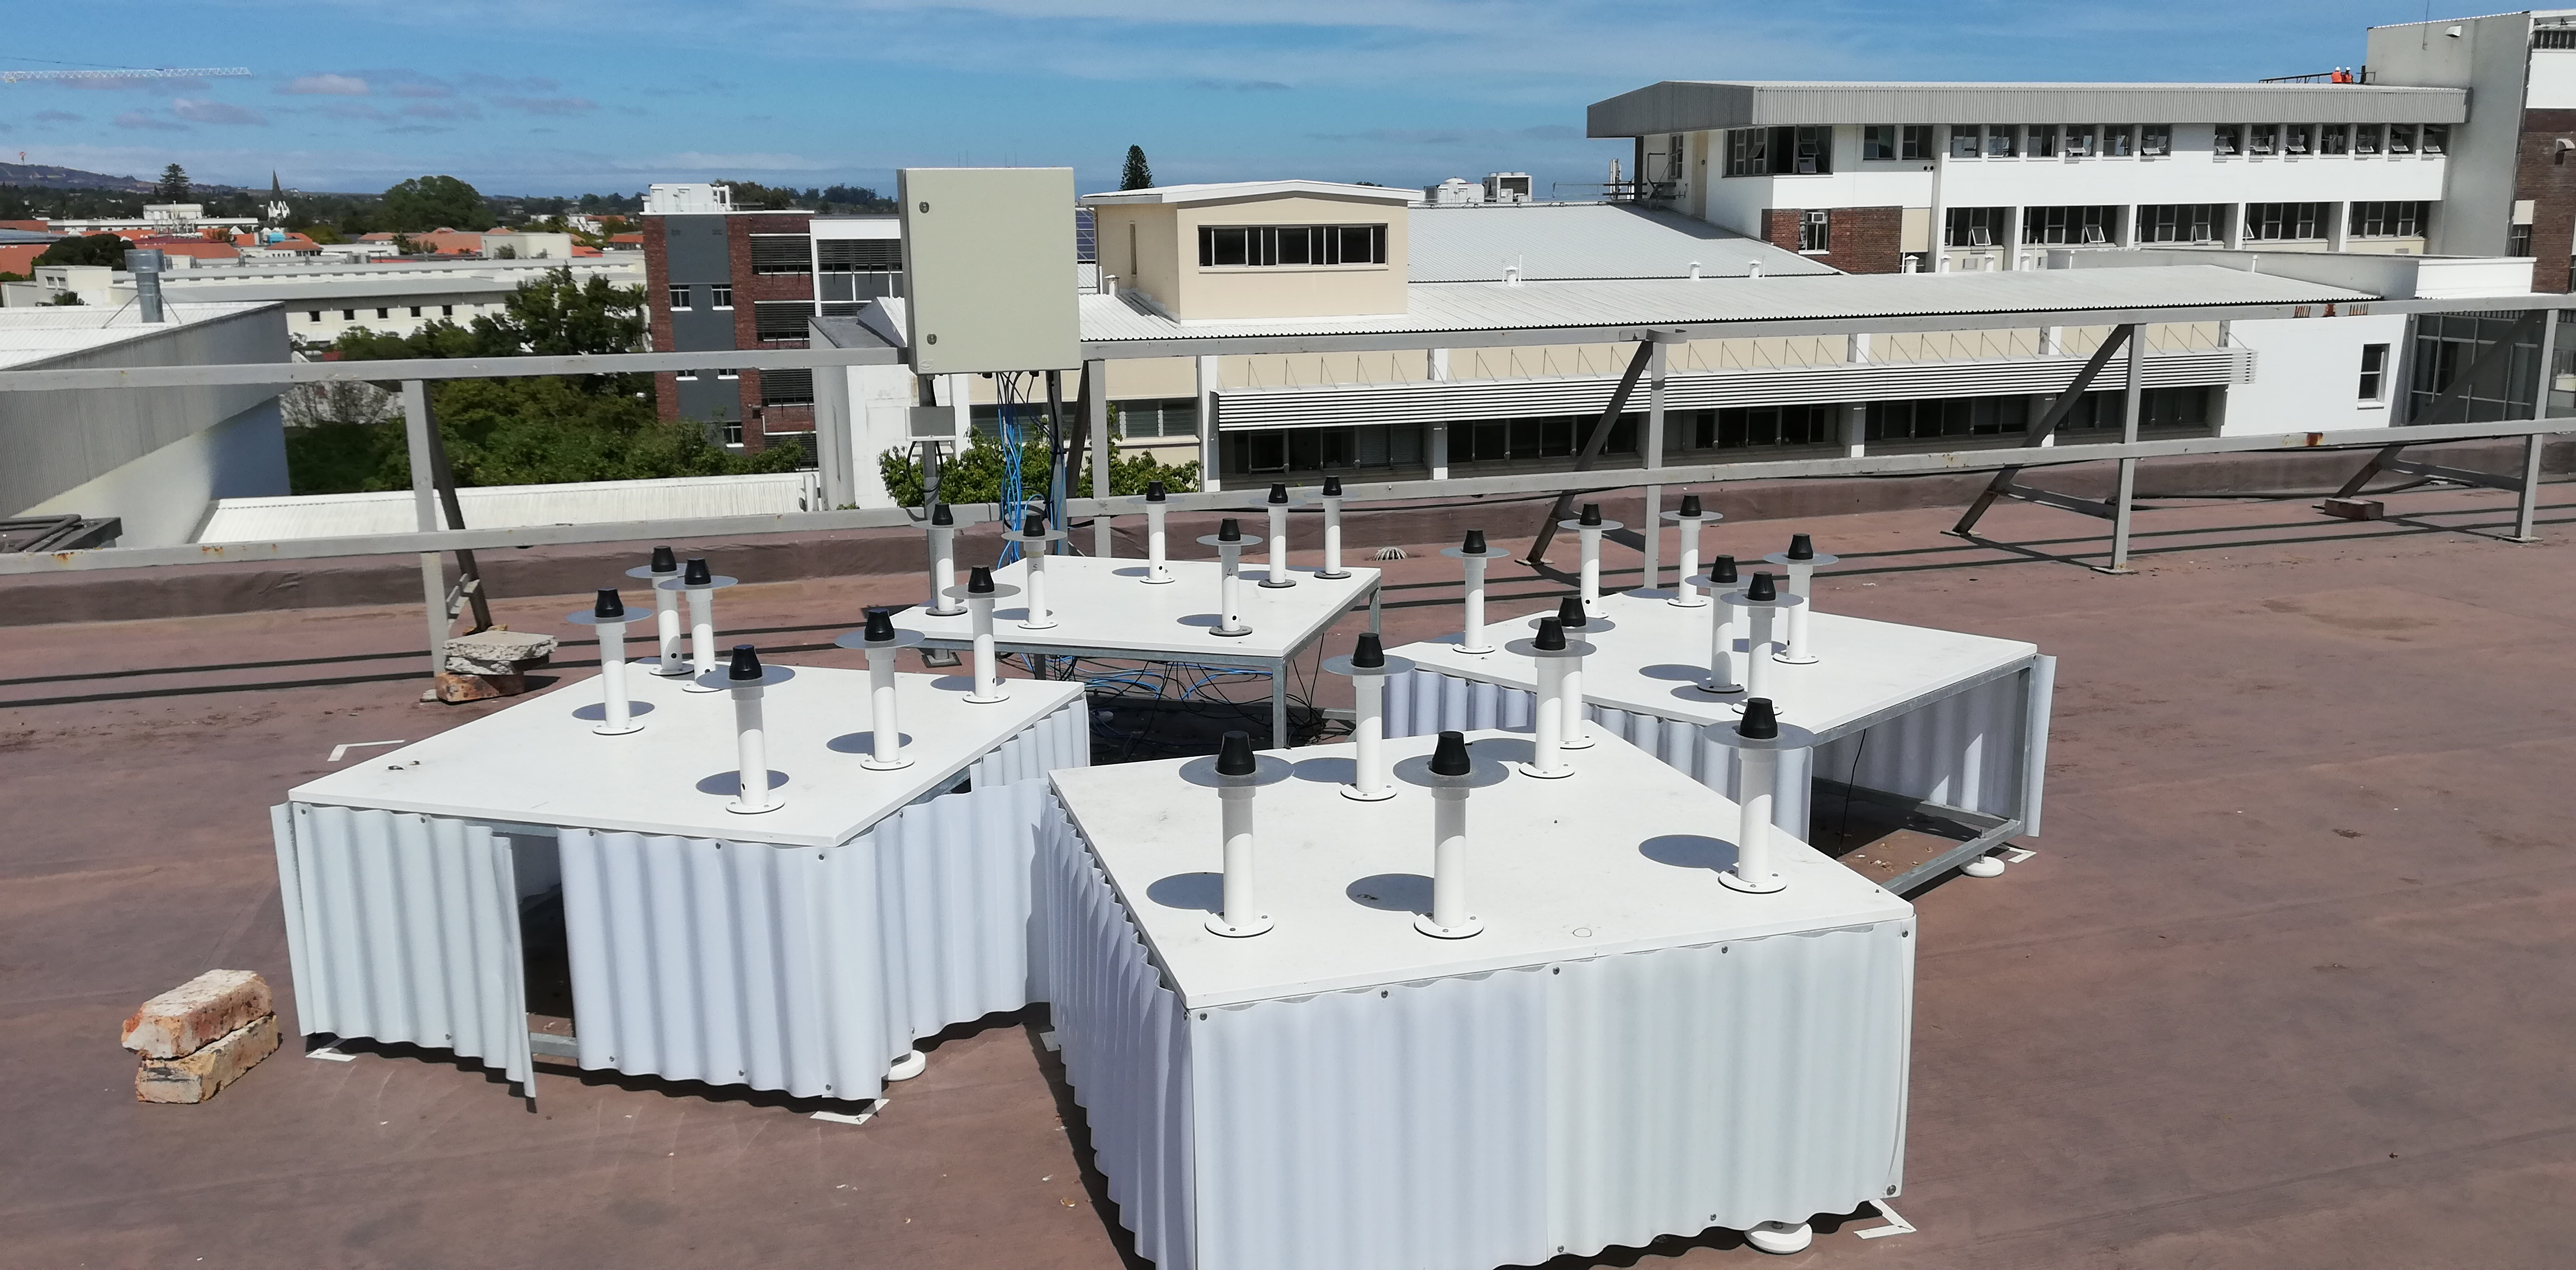
\includegraphics[scale=0.08]{images/TART.jpg}
    \caption{The TART deployed on top of the Electrical Engineering building}
    \label{fig:TART}
\end{figure}